% Chapter 2 - Background

% \glsresetall % reset the glossary to expand acronyms again
\chapter[Background]{Background}\label{ch:CH2-Background}
\index{Background}

\gls{ML} and \gls{DL} are groundbreaking technologies set to shape the near future, and there will be immense demand to run them at scale on \gls{HPC} systems.
This chapter will establish the fundamentals of \gls{HPC} from the bottom up.
It starts with a deep dive into the node architecture, discussing the trend of heterogeneous clusters, then scaling up to the system level to evaluate the technologies interconnecting all the compute islands.
Next, the software environment is established, since this thesis is focused on communication libraries, we start with 'transport-layer' libraries which are used to build \gls{MPI} implementations, then we discuss \gls{MPI} itself, why it is prevalent, and its essential features. 
Lastly, we define topology awareness and \gls{PAP} awareness, as they are the fundamental ideas used to propose new algorithms in Chapters \ref{ch:CH4-TopologyAwareness} and \ref{ch:CH5-PAPAwareness}.

\section{GPU Cluster Architectures}
Modern \gls{HPC} is performed on \gls{GPU} clusters, which are essentially a bunch of nodes (rack-mounted servers with \gls{GPU}s), tied together through an ultra-high-performance \gls{SAN}.
These machines are assembled using commodity parts, and system designers can integrate components from different vendors.
The fundamental components include the \gls{CPU}, \gls{GPU}s, and the interconnect, all of which have different vendors providing different solutions with their own price/performance/density tradeoffs.
This provides a lot of freedom in system design, allowing system designers to optimize across multiple factors, including density, scalability, power consumption, and cost.
While system designers have flexibility in their deployments, several foundational concepts and technologies are consistent across the most powerful systems.

The components in a cluster can be grouped into two categories: they perform compute or move data between computing endpoints.
Both \gls{CPU}s and \gls{GPU}s can perform compute within a compute node, and there are interconnects like \gls{PCIe} and NVLink that shuffle data between compute resources.
At a larger scale, each node can be considered a compute island while the network shuffles data between nodes.
Each resource has its quirks, and applications need to be designed appropriately to make full use of system resources, and at the same time, it is the library designer's job to provide tools that efficiently expose the granularity of control that developers need without overwhelming them with hardware details.

An additional category of components is focused on accelerating file I/O.
These components can include node-local \gls{SSD} or Intel's Optane persistent memory \cite{Weiland2019EvalOfOptaneForSciApps}. 
They are used to expose a higher-performance file system with better bandwidth and latency than traditional network-attached storage.
While these tools are essential, and many applications are file I/O bound, these tools are out of the scope of this thesis. 

\subsection{Compute Node Architecture}
The compute nodes are where the calculations happen.
A compute node's primary design goal is to perform as many \gls{FLOPS} as possible while minimizing power consumption and area.
At a high level, a node can be thought of as a rack in a server tying together memory, \gls{CPU}s, \gls{GPU}s, network cards, and maybe a bit of local storage, but there is nuance to node design and tradeoffs that determine component selection. 

\subsubsection{CPU Compute Nodes}
Traditionally, compute nodes would be entirely \gls{CPU} based, with one or more sockets per node.
Typical \gls{CPU} nodes can have 32 to 128 cores per node depending on the \gls{CPU} model, and each \gls{CPU} has their own memory controllers attached to a pool of memory ranging from 128GB to over 4TB.
Thanks to the operating system technology, multiple \gls{CPU} sockets are combined and presented to applications as a single giant \gls{CPU} attached to a massive pool of memory. 
Processes running on any core can access memory from any memory bank attached to any other \gls{CPU}.

This model is known as a \gls{SMP}, where processes share a common memory bus, and any thread can access any other process' memory, but in reality, these systems are not exactly symmetric.
Since each socket has its own memory controllers, each socket has its own \gls{NUMA} domain, and there is a performance penalty accrued when cores access memory in other process's \gls{NUMA} domains.
There are also complex cache hierarchies, and if two cores are frequently modifying the same memory location, the contention caused by frequent cache flushes will tank performance, this is also known as cache thrashing.
So when writing parallelized code, application developers must consider where data resides in memory and how \gls{CPU} cores access that data.
 
The number of cores in \gls{CPU}-based \gls{NUMA} architectures has been growing over the past decade, with high-end systems topping out around 128 cores (256 if you consider hyperthreading).
The trouble with modern \gls{CPU} cores is that they are complicated.
The x86 instruction set has been around since the 80s and has been expanded multiple times; there are \gls{SIMD} instructions for vectorization, extensions targeting security-critical applications, and even compatibility modes for older 32-bit programs. 
There are alternate RISC \gls{ISA} that cut down on instruction complexity, with the most mature being ARM, but these cores are still fairly large and optimized for single-thread compute.
\gls{CPU} cores tend to be large and not very space efficient, limiting the number of cores per node, but there are new technologies that leverage much smaller cores to build much more parallel chips. 

\subsubsection{GPU Compute Nodes}

\gls{GPU}s subvert the core-complexity problem of \gls{CPU}s by greatly simplifying the core design and providing thousands of cores per chip. 
These accelerators provide massively parallel banks of floating-point compute, and they can perform so many \gls{FLOPS} they require specially manufactured \gls{HBM} to saturate compute-core utilization.
In terms of \gls{FLOPS}/mm$^2$ and \gls{FLOPS}/Watt, \gls{GPU}s win out by orders of magnitude, which is one of the most prominent driving reasons why \gls{GPU} adoption for compute-intensive applications has exploded over the past decade.
You can also associate multiple \gls{GPU}s to a single \gls{CPU}, so the trend has been to pack as many \gls{GPU}s into a node as possible.
When \gls{GPU}s first took first place on the Top500 with Titan at \gls{ORNL}, there was a single \gls{GPU} per node, but a decade later, Frontier has scaled up to eight \gls{GPU}s per node (technically, there are four MI250x cards per node, but each card has two \gls{GPU} dies tied together with some advanced packaging solution, and it is presented to the application as eight \gls{GPU}s).

But, these external accelerators also add considerable amounts of complexity to system design, and that complexity is felt most acutely at the software level.  
Because \gls{GPU}s are fundamentally different from \gls{CPU}s, they require special programming models.
Programmers specify \gls{GPU}-bound parallel computations in a \gls{GPU} kernel, and kernels are launched simultaneously across a user-specified number of threads at run-time.
To save die space, \gls{GPU} cores discard bloat, like branch predictors, so control flow inside compute kernels can destroy performance if not accounted for properly.
Since thousands of threads can run simultaneously, even more attention has to be paid to memory access patterns, as there is even more potential for poorly optimized code to tank performance (see memory coalescing \cite{CUDAMemCoalescing}).
There is also the fact that \gls{GPU}s have their own \gls{HBM} that load/store \gls{CPU} instructions can not access, and \gls{GPU} kernels can only access data resident to the card they are running on, so device data management is another challenge developers need to account for. 
But when everything comes together, when memory accesses are coalesced, when there is no warp divergence, when \gls{CPU}-\gls{GPU} memory transfers are overlapped with compute, \gls{GPU}s can be orders of magnitude faster than \gls{CPU}s.

\subsubsection{Interconnects}\label{sec:CH2-interconnects}
Within a node, like the one depicted in Figure \ref{fig:nvidia_redstone}, there are many places data can reside.
Data can sit in host memory or device memory, host memory can be further subdivided into \gls{NUMA} domains, and there are often multiple \gls{GPU}s with their own memory domains.
So data is constantly being shuffled between different types of memory, and to accommodate this, the hardware interconnecting different memory regions needs to be as fast as possible.
Several technologies have been designed to support these operations, with broad categories including cross-socket \gls{CPU}-\gls{CPU} interconnects, host-to-device interconnects, and  \gls{GPU}-\gls{GPU} interconnects.

\begin{figure}
    \centering
    \begin{tikzpicture}[
        gpusty/.style={draw, rectangle,
            minimum height=1cm,
            minimum width=1cm,
            fill=lime!70!black
        },
        cpusty/.style={draw, rectangle,
            minimum height=1cm,
            minimum width=1cm,
            fill=blue!70
        },
        memsty/.style={draw, rectangle,
            minimum height=0.6cm,
            minimum width=1cm,
            fill=black!20
        },
        nicsty/.style={draw, rectangle,
            minimum height=1cm,
            minimum width=1cm,
            fill=purple!70
        },
        darrowsty/.style={draw, double arrow,
            fill=lime!30!white,
            font=\footnotesize,
        },
        memarrowsty/.style={draw, double arrow,
            minimum height=1cm,
            minimum width=0.6cm,
            fill=black!40,
            font=\footnotesize,
            rotate=90,
        }
    ]
    
    \node[gpusty] at (-1.7,-1.5) (g0) {GPU0};
    \node[gpusty] at (1.7,-1.5) (g1) {GPU1};
    \node[gpusty] at (-1.7,1.5) (g2) {GPU2};
    \node[gpusty] at (1.7,1.5) (g3) {GPU3};
    
    \node[nicsty] at (-3.5, 0) (n) {NIC};

    \node[cpusty] at (-1.5, 3.5) (c0) {CPU0};
    \node[cpusty] at (1.5, 3.5) (c1) {CPU1};
    
    \node[memsty] at (-1.2, 5.1) (m0) {NUMA0};
    \node[memsty] at (1.2, 5.1) (m1) {NUMA1};

    \node[darrowsty, minimum height=2cm] at (0,-1.5) () {NVLink};
    \node[darrowsty, minimum height=2cm] at (0,1.5) () {NVLink};
    \node[darrowsty, rotate=90, minimum height=2.1cm] at (-1.5, 0) () {NVLink};
    \node[darrowsty, rotate=90, minimum height=2.1cm] at (1.5, 0) () {NVLink};
    \node[darrowsty, rotate=45, minimum height=3cm] at (0,0) () {NVLink};
    \node[darrowsty, rotate=-45, minimum height=3cm] at (0,0) () {NVLink};

    \node[draw, double arrow, 
        minimum height=1cm,
        fill=blue!40,
    ] at (0, 3.5) () {UPI};
    
    \node[memarrowsty] at (-1.2, 4.4) () {};
    \node[memarrowsty] at (1.2, 4.4) () {};

    \draw[<->] (n) -- (-3.5,3.5) node[above]{PCIe x16} -- (c0) ;
    \draw[<->] (g0) -- (-2.7,-1.5) -- (-2.7,2.7) -- (-1.8, 2.7) -- (c0.240);
    \draw[<->] (g2) -- (-1.7,2.5) -- (-1.2, 2.5) -- (c0.300);
    \draw[<->] (g1) -- (2.7,-1.5) -- node[below,sloped] {PCIe x16} (2.7,2.7)  -- (1.8, 2.7) -- (c1.300);
    \draw[<->] (g3) -- (1.7,2.5) -- (1.2, 2.5) -- (c1.240);
    
    \end{tikzpicture}
    \caption[Topology of Multi-GPU Node]{
    Sample architecture for GPU node.
    There are 4 GPUs fully connected with NVLink device-to-device interconnects. 
    The GPUs are connected to the CPU through PCIe, with each CPU managing 2 GPUs. 
    The network card is also attached to the CPU0 with PCIe.}
    \label{fig:nvidia_redstone}
\end{figure}


For multi-socket shared-memory systems to work correctly, a hardware mechanism must be implemented to maintain memory and cache coherency between the \gls{CPU}s.  
The technology behind these solutions is often proprietary and vendor-specific, with each \gls{CPU} vendor having their own implementation.
For example, Intel's Xeon Scalable processors can be connected through \gls{UPI} \cite{XeonTechOverview}.
Xeon \gls{CPU}s have two or three \gls{UPI} links depending on the \gls{CPU} model, which can transfer data at 10.4GT/s and can be combined into different topologies of two, four, or eight \gls{CPU}s.
Intersocket link designs are often tightly coupled to the on-chip memory controllers, seeing as their job involves connecting said memory controllers across sockets.
These interfaces strive to be transparent to applications, so programming for these interfaces is not that explicit. 
It often involves critically thinking about thread/process-to-core bindings and ensuring compute kernels are not cache thrashing.

To move data in and out of accelerator memory, systems leverage \gls{PCIe}.
The \gls{PCIe} standard, maintained by the PCI-SIG consortium, was first released in 2003 and has evolved over the years to meet ever-increasing communication needs \cite{PCIeIntroPaper, PCIeV5Spec}.
A \gls{PCIe} connection is based on a scalable number of lanes, representing the physical wires connecting the endpoints, and can range from a single lane up to 16 lanes, with more lanes providing more bandwidth.
At the time of writing, the most common implementation is \gls{PCIe} V4 which provides bidirectional 2GB/s per lane, letting high-performance devices top out at 32GB/s on a 16x connection. 
\gls{PCIe} is also a switched architecture, for example, it is possible to design a system where a 16x connection coming off the \gls{CPU} can be passed into a switch and connected to four \gls{GPU}s with their own 16x endpoints.
This type of design allows \gls{CPU}s with limited \gls{PCIe} lanes to connect more devices yet imposes performance restraints on said devices since they all need to share a single host connection.
The \gls{PCIe} standard is not just for accelerators, it is designed to work for any I/O device and is also used to connect storage devices and network cards to the \gls{CPU}.
Many operations traverse \gls{PCIe} transparently since the implementation is handled by device drivers, for example, all network operations cross \gls{PCIe}, and all file I/O operations pass a \gls{PCIe} connection, both for local storage and network attached storage.
In most \gls{GPU} programming models, the host-to-device transfers are explicit through functions like \texttt{cudaMemcpyAsync}, so developers will know when transfers are taking place and can use techniques like compute-communication overlap to hide transfers.

The last category of connections is \gls{GPU} to \gls{GPU} interconnects, and there are several technologies here, both proprietary and open.
Initially, if a system had multiple \gls{GPU}s, transfers would have to be staged through host memory, but \gls{GPU}s can also send data to each other through \gls{PCIe} peer-to-peer.
This technology cuts host memory out of the data's path, increasing bandwidth and freeing up \gls{CPU} resources to handle other tasks.
But the pace of development for \gls{PCIe} is relatively slow since consortiums are not quick in publishing new standards. 
Since PCI-SIG can not keep up with the scaling bandwidth requirement of \gls{HPC}, \gls{GPU} manufacturers have started to create their own device-to-device connections.
For example, Nvidia's \gls{GPU}s can leverage NVLink.
NVLink3, the third generation of NVLink announced alongside the A100 \gls{GPU}, can transmit data at 50Gb/s per lane and has an accompanying NVSwitch for scalability \cite{Foley2017PascaleAndNVLink}.
Each A100 \gls{GPU} has 12 links, allowing system designers to build different topologies.
For example, four \gls{GPU} nodes can have a fully-connected topology with each \gls{GPU} connected by a 200Gb/s pipe, or an ultra-dense eight \gls{GPU} node can leverage six NVSwitches in parallel to build a star topology.
These connections can be orders of magnitude faster than \gls{PCIe} and are tightly integrated with the \gls{GPU}s memory controller.
Programmatically, developers drive NVLlink through cudaIPC, a model similar to mapped memory where a memory handle from one \gls{GPU} is passed to another \gls{GPU} through main memory, then compute kernels can access the remote memory region as if it is local memory.

\subsection{The Network}
The last and most critical piece of a cluster is the network.  
A single node will have some inherent scalability limit, often bottlenecked by compute (number of \gls{CPU} cores or \gls{GPU}s) or memory (the number of memory channels the \gls{CPU} can support or the available \gls{GPU} memory).
\gls{HPC} Clusters break this limit by tying multiple nodes together through a high-bandwidth and low-latency network so that programmers can scale their application across the resources of multiple nodes.
But once again, adding this extra layer for scalability adds a much higher complexity that needs to be accounted for.

The network topology describes how the nodes are connected, it is often modelled as a graph where vertices are either nodes or switches, and edges represent the network links connecting resources.
In the past, large systems would deploy switchless fabrics, with popular topologies including mesh and torus networks.
Some production clusters still use switchless networks as they map well to the communication patterns of specific \gls{HPC} applications, but modern commodity hardware has converged on switched topologies, as they are easier to deploy, scale, and manage. 
There are many switched topologies used in practice and proposed in the literature, popular ones include Clos and dragonfly, but the most common switched topology deployed in \gls{HPC} clusters is fat-tree.
A sample fat-tree topology with 16 nodes and two levels is demonstrated in Figure \ref{fig:fat-tree-topology}, similar to a tree data structure, there is a spine switch (the root of the tree) connected to leaf switches (children of the root) which connect to the nodes (leaves of the tree).
Fat-tree gets its name because links at the top of the tree will have more bandwidth than links at the bottom.
This design feature is because all nodes can potentially send data across the root simultaneously, meaning the spine switch can be subject to much more demand than leaf switches.
To save costs, fat trees can be designed with a blocking factor which describes the ratio of available bandwidth at the root compared to the number of children attached to a leaf node.
A non-blocking fat-tree can afford to have all nodes send data across the root simultaneously, while a tree with a 5:1 blocking ratio will grind down to 1/5 of the potential bandwidth if all processes go through the spine at the same time.

\begin{figure}
    \centering
    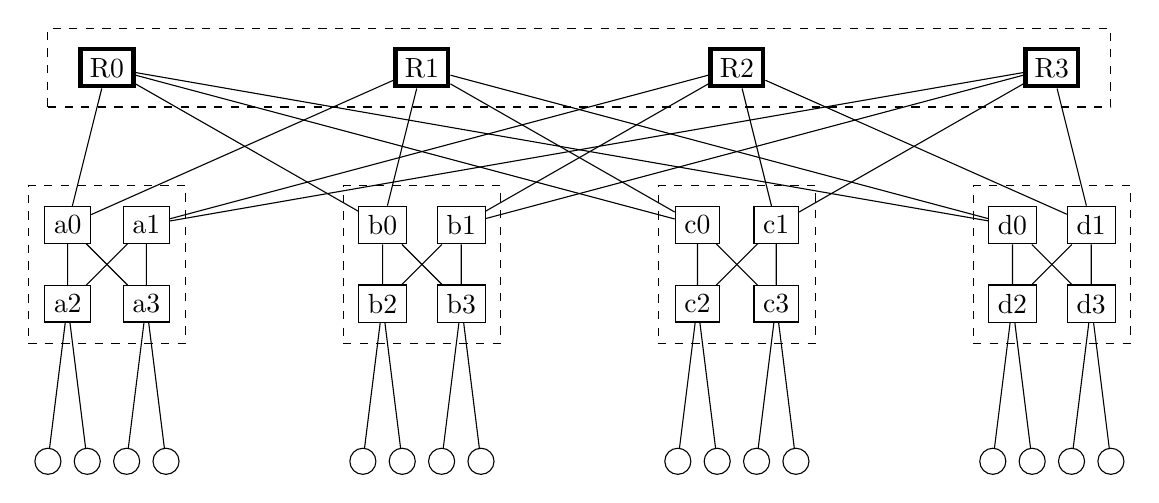
\begin{tikzpicture}[
        nsty/.style={circle,draw,font=\large},
        ssty/.style={font=\LARGE},
        rswsty/.style={rectangle,draw,ultra thick},
        lswsty/.style={rectangle,draw},
        nsty/.style={circle,draw,font=\tiny},
    ]
    \foreach \o/\l in {0/a,4/b,8/c,12/d}{
        \node (b\o) at (\o+0.75, 2.5) [rectangle, draw, dashed,
            minimum width=2cm, minimum height=2cm] {};
        \node (s\o0) at (\o+0.25, 3) [lswsty] {\l0};
        \node (s\o1) at (\o+1.25, 3) [lswsty] {\l1};
        \node (s\o2) at (\o+0.25, 2) [lswsty] {\l2};
        \node (s\o3) at (\o+1.25, 2) [lswsty] {\l3};
        \foreach \x in {0,1,2,3} {
            \node (n\o\x) at (\x/2+\o, 0) [nsty] {};
        }
        \draw (s\o0) -- (s\o2) -- (n\o0);
        \draw (s\o0) -- (s\o3) -- (n\o2);
        \draw (s\o1) -- (s\o2) -- (n\o1);
        \draw (s\o1) -- (s\o3) -- (n\o3);
    }
    \node (r0) at (0.75,5) [rswsty] {R0};
    \node (r1) at (4.75,5) [rswsty] {R1};
    \node (r2) at (8.75,5) [rswsty] {R2};
    \node (r3) at (12.75,5) [rswsty] {R3};
    \node () at (6.75, 5) [rectangle, draw, dashed,
            minimum width=13.5cm, minimum height=1cm] {};
    \foreach \i in {0,4,8,12}{
        
        \draw[] (r0) -- (s\i0);
        \draw[] (r1) -- (s\i0);
        \draw[] (r2) -- (s\i1);
        \draw[] (r3) -- (s\i1);
    }
    \end{tikzpicture}
	\caption[Sixteen-Node Two-Level Fat Tree Network]{
        Sample non-blocking fat-tree network connecting 16 nodes.
        The network uses 4-port switches, but combines them into groups to create leaf/root switches.
        The top row of switches encompass the root of the network, and the groups of four switches in the middle are the leaf switches. 
     }
	\label{fig:fat-tree-topology}
\end{figure}


In \gls{HPC} communities, the most widely adopted type of network is InfiniBand. 
InfiniBand is a networking standard published by the \gls{IBTA} \cite{IBSpec}.
The first InfiniBand spec was published in 2001 with hardware that could support speeds around two Gb/s, but over time the standard and technology have evolved, and now modern InfiniBand networks can transfer data at 400 Gb/s.
The other key characteristic of an \gls{HPC} network is tremendously low latency, and network designers have poured years into removing any possible overhead from the communication code path. 
Key technologies include, but are not limited to, kernel bypass, hardware tag matching, and network offload.
The InfiniBand specification outlines both the network hardware's physical characteristics and the InfiniBand verbs programming interface \cite{IBSpec}.
InfiniBand is not the only programming interface, though, and many players have moved in and out of the \gls{HPC} networking market.
Cornelis Networks develops OmniPath \cite{Birrittella2015OmniPath}, and Cray has their line of SlingShot networks \cite{DDeSensi2020InDepthAnalysisOfSlingshot}, all of which share similar performance and foundational ideas in their design but differ enough to fall across a diverse price/performance spectrum.

\section{Communication libraries} 
\begin{figure}
    \centering
    \begin{tikzpicture}[
        botsty/.style={
            draw, rectangle, fill=black!30,
            minimum height=1cm,
            minimum width=3cm,
            font=\large
        },
        libfabsty/.style={
            draw, rectangle, fill=blue!20,
            minimum height=2.5cm,
            minimum width=5.5cm,
        }, 
        libfabitemsty/.style={
            draw, rectangle, fill=blue!40,
            minimum height=1.3cm,
            minimum width=2cm,
            align=center,
            font=\footnotesize,
        }, 
        ucxsty/.style={
            draw, rectangle, fill=orange!20,
            minimum height=4cm,
            minimum width=5.5cm,
        },        
        ucxitemsty/.style={
            draw, rectangle, fill=orange!40,
            minimum height=1.3cm,
            minimum width=2cm,
            align=center,
            font=\footnotesize,
        }, 
        ncclmainsty/.style={
            draw, rectangle, fill=green!30,
            minimum height=2.5cm,
            minimum width=3cm,
        },
        ncclitemsty/.style={
            draw, rectangle, fill=green!50,
            minimum height=1.3cm,
            minimum width=2cm,
            align=center,
            font=\footnotesize,
        },
        mpiitemsty/.style={
            draw, rectangle, fill=black!10,
            minimum height=1.3cm,
            minimum width=2cm,
            align=center,
            font=\footnotesize,
        }
    ]

    \node[botsty] (0,0) (GPUd) {GPU drivers};
    \node[botsty] (shmem) [right=0.9cm of GPUd] {shared mem};
    \node[botsty] (verbs) [right=0.9cm of shmem] {IB verbs};
    \node[botsty] (NICd) [right=0.9cm of verbs] {NIC drivers};
    
    \node[libfabsty] (libfabmain) [above=0.3cm of GPUd, xshift=1.25cm] {};
    \node[font=\large] (libfabtitle) [below=0.2cm of libfabmain.north] {Libfabric};
    \node[libfabitemsty] (libfabdd) [above=0.3cm of libfabmain.223] {Device\\Discovery};
    \node[libfabitemsty] (libfabtrans) [right=0.5cm of libfabdd] {Data\\Transmission};
    
    \node[ucxsty] (ucxmain) [right=0.5cm of libfabmain, yshift=0.75cm] {};
    \node[font=\large] (libfabtitle) [below=0.2cm of ucxmain.north] {UCX};
    \node[ucxitemsty] (ucxts) [above=0.2cm of ucxmain.240] {Transport\\Selection};
    \node[ucxitemsty] (ucxtrans) [right=0.3cm of ucxts] {Data\\Transmission};
    \node[ucxitemsty] (ucxdm) [above=0.3cm of ucxts] {Device\\Management};
    \node[ucxitemsty] (ucxmr) [right=0.3cm of ucxdm] {Topology\\Detection};

    \node[draw, rectangle, fill=yellow!40, font=\large,
            minimum height=0.5cm,
            minimum width=6cm,
    ] (ucc) [above=0.3cm of ucxmain.50, xshift=1.5cm] {UCC};
    
    \node[ncclmainsty] (ncclmain) [right=0.4cm of ucxmain.15, font=\large] {};
    \node[below=0.2cm of ncclmain.north, font=\large] {NCCL};
    \node[ncclitemsty] (ncclcoll) [above=0.3cm of ncclmain.south] {GPU Optimized\\Collectives};

    \draw (-1.5,3.7) -- ++(5.5,0) -- ++(0,1.3) -- ++(3,0) -- ++(0,1) -- ++(6.5,0) -- ++(0,2.9) 
        -- node[midway, below, font=\large]{MPI} ++(-15,0) -- (-1.5, 3.7);
        
    \node[mpiitemsty] (mpids) [above=1.1cm of libfabmain.137] {Device\\Selection};
    \node[mpiitemsty] (mpift) [above= of mpids] {Fault\\Tolerance};
    \node[mpiitemsty] (mpidtype) [right=0.8cm of mpift] {Datatype\\Engine};
    \node[mpiitemsty] (mpivt) [right= 0.8cm of mpidtype] {Virtal\\Topologies};
    \node[mpiitemsty] (mpiprocmgmt) [right=0.8cm of mpivt] {Process\\Management};
    \node[mpiitemsty] (mpitd) [right=0.8cm of mpiprocmgmt] {Topology\\Detection};
    \node[draw, rectangle, fill=black!10, font=\footnotesize,
        minimum height=0.6cm,
        minimum width=5cm,
    ] (mpicoll) [right=0.7cm of mpids.north east, yshift=-0.3cm] {Collective Communication};

    \node[draw, rectangle,
        minimum width=15cm,
        font=\large,
        fill=black!30
        ] (apps)[above=1.1cm of mpivt, xshift=0.5cm] {Applications (Horovod, Gadget, NEK5000, Trilinos, PETSc)};
    
    \end{tikzpicture}
    \caption[MPI Software Stack]{
        The division of responsibilities for MPI software in HPC systems.
        The MPI layer provides tools for process orchestration and communication.
        MPI implementations often call into either Libfabric or UCX to access network resources. 
        External collective libraries like NCCL and UCC can also be leveraged for collective communications.
    }
    \label{fig:hpc_software_arch}
\end{figure}
There are limits to how applications can interact with the network.
Modern networks have message latencies on the order of microseconds, but compared to L1 cache latencies being on the order of nanoseconds, network transfers are excruciatingly slow.
With drastic performance limits that need to be designed around and a diverse set of network hardware to choose from, a unique set of programming tools are required to expose network resources. 
There are vast differences in vendor technology as well, different networks have different software layers built on top of them, and portability between networks is an essential requirement for many applications. 
So over time, a series of \gls{API}s have formed, each targeting different types of users, exposing more/less granularity of the hardware and various types of convenience functions designed to help write code for each layer.
Figure \ref{fig:hpc_software_arch} outlines the common structure and division of responsibilities found in HPC software.
The lowest layer would be device-specific libraries, these are vendor-specific data structures and functions designed to interact directly with hardware on the network card.
Above the device layer would be the transport layer, these are \gls{API}s designed to wrap around different communication endpoints; they are still not that user-friendly, but they provide more portability and can more easily manage different sets of resources.
The transport layer is used to build programming models, with the most common model being \gls{MPI}.
This is the layer application developers are expected to interact with since it provides the most flexibility and portability for scientific codes.

\subsection{Device APIs and the Transport Layer}

The lowest possible layer of network software are device-specific interfaces. 
Each vendor has their own, for example, InfiniBand has verbs \cite{IBSpec}, Cray's Aries interconnect has \gls{GNI} \cite{Choi2015ImplOfOFILibfabricGNI}, and Intel/Cornellis Netwoks' OmniPath has \gls{PSM2} \cite{IntelPSM2ProgGuide}.
These \gls{API}s are often tightly coupled to device drivers and directly manage memory and registers on the network card.
There are often two types of data transfer models: two-sided and one-sided communication.
The two-sided model can be thought of as point-to-point messages, applications post send messages indicating which buffers to move to across the network, and the remote peer posts a receive buffer indicating where to place the data.
This model heavily corresponds to \texttt{MPI\_send}/\texttt{MPI\_recv}, and network cards often have hardware built in specifically to handle parts of this \gls{API}.  
The one-sided model, often referred to as \gls{RDMA}, cuts out the involvement of the remote process.
The remote peer registers a memory region, and the communicating processes can put/get data in that region without remote \gls{CPU} involvement.
Network cards will also provide atomic memory operations like compare-and-swap and fetch-and-increment.
While semantically similar to assembly instructions with the same name, these endpoints perform their function in remote memory.
These one-sided functions loosely map to \gls{MPI}'s \gls{RMA} \gls{API}, as well as other one-sided programming models like \gls{UPC} and SHMEM.

Device \gls{API}s are the most performant layer, as they are as close as possible to the hardware, but they are often difficult to use and not portable at all.
This is where the transport layer comes in, with the two most well-known interfaces being Libfabric and \gls{UCX}.
Transport layer libraries provide a programming model that can be easily mapped to multiple types of hardware but still be abstract and portable enough so that vendors can add/remove features specific to their hardware.
When instantiating a libfabric endpoint, users explicitly choose the type of network they want to establish, and options can include sockets, shared-memory, vendor-specific transports, and many more.
So libfabric provides an abstraction of the network resources, some registration routines, and a work queue-based communication model for one-sided and two-sided communications \cite{libfabric}.
In the work queue model, processes post communication requests on a work queue and poll a corresponding completion queue for communication completion, the benefit of this model is that it maps very closely to how the hardware works.
One issue with libfabric is that higher-level programming models still have to manage multiple types of resources to ensure that the proper hardware is used for the appropriate transactions. 
However, \gls{UCX} avoids this problem by handling transport selection.
\gls{UCX} provides similar abstractions for network resources, memory registration and one/two-sided communication, but the communication model is based on callbacks to notify completion \cite{shamis2015ucx}.
This callback-based model provides more flexibility to user implementation at the cost of increased overhead.
While their completion models differ, both support point-to-point messages (tagged and untagged) and one-sided operations, and both communication models are frequently used by higher-level libraries or have hardware optimizations built into high-performance network cards.
Both libraries also support (or at least specify support for) accelerators, this means it is possible to pass \gls{GPU} buffers into communication operations and expose device memory for \gls{RDMA}.

These interfaces are friendlier and provide nicer and more portable endpoints than vendor \gls{API}s. 
However, they still have a lot of rough edges, and the target audience is systems developers, not domain scientists.
Transport layer libraries often expect users to perform a lot of memory and device management, which can place a lot of unnecessary burdens on application developers.
That is why there is one more layer above the transport layer, the programming model layer, which is intended to be used by a more science-focused audience.

\section{The Message Passing Interface}
At the highest level, application developers are expected to use a programming model to build their scientific apps. 
While there are multiple types of distributed memory programming models, \gls{MPI} is by far the most prevalent and widely used.
The MPI-Forum \cite{MPIForum}, the academic/industry body responsible for standardizing \gls{MPI}, is often a bridge between the application community and the networking community.
The first \gls{MPI} specification was released in 1994 and started as a two-sided programming model with support for collective communications, and has evolved with MPI-2, published in 1997, adding support for a one-sided programming model.
The latest spec, MPI-4, specifies many more features like neighbourhood collectives, partitioned communication, virtual topologies, datatype management, distributed I/O and more.

\gls{MPI} is a programming model for multi-process distributed memory programming, so at program launch, each process needs to be created by a call to \texttt{fork()}, and connection information (including but not limited to hostname and PID) needs to be distributed among all processes. 
Process creation is handled by \texttt{mpiexec}, a program \gls{MPI} implementations must provide. 
Users can specify how many processes to launch, how to bind processes to resources, and the executable file's location.
Inside the user's code, the first \gls{MPI} routine that must be called is \texttt{MPI\_Init()}, which is responsible for instantiating the \gls{MPI} library, and performs tasks like network card initialization and wireup.
One of the data structures \texttt{MPI\_Init()} sets up is the global communicator \texttt{MPI\_COMM\_WORLD}, communicators are a structure encapsulating a set of processes that can exchange data with each other, and \texttt{MPI\_COMM\_WORLD} contains every process launched by \texttt{mpiexec}.
Each process in a communicator is assigned a rank, a unique identifier ranging from zero to the size of the communicator minus 1. 
These ranks are used to identify an individual process within a communicator.
\texttt{MPI\_Init()} instantiates the global communicator, but applications can create new communicators to carve out smaller groups of processes or renumber processes to map to a topological structure.

To comprehend why \gls{MPI} is so powerful, it is necessary to understand \gls{MPI}'s message-passing model, this interface specifies how two processes exchange data.
Point-to-point messages can be extended to a collective model where multiple processes exchange data in a pre-determined manner.
Collective communication routines are extremely powerful and heavily relied upon in practice.
Further, understanding the one-sided model is also essential, as it provides tools for managing communication without peer involvement.

\subsection{Two-Sided Communication}
The two-sided model is built around sending and receiving messages across a communicator.
Messages are specified as a vector of \gls{MPI} datatypes, which can vary from a simple array of integers to complex structures of derived datatypes.
\texttt{MPI\_Send()} specifies a segment of data to send to a remote process, and the remote process must post a corresponding \texttt{MPI\_Recv()} indicating where the data will be placed. 
The send operation identifies the destination through a tuple containing a rank, tag, and communicator, the corresponding receive must match these fields or have wildcard values for \texttt{MPI\_ANY\_SOURCE} or \texttt{MPI\_ANY\_TAG}.

However, there are nuances to using the message-passing model.
Messages are non-overtaking, so if two back-to-back sends can match the same receive, then the first message needs to complete before the second.
Standard \gls{MPI} operations are blocking, this means program execution can halt at a communication call until the operation is complete.
If the programmer is not careful, poorly written code can waste millions of cycles doing nothing, waiting for other nodes to complete.
Furthermore, it can also lead to deadlocks.
If a process gets stuck in a blocking receive that does not have a corresponding send, the program will hang.

In a later version of the \gls{MPI} specification, non-blocking messages were introduced with corresponding \texttt{MPI\_Isend()}/\texttt{MPI\_Irecv()} functions.
These endpoints return immediately but do not complete communication; instead, they populate an \texttt{MPI\_Request} object with information about the ongoing communication.
The programmer needs to progress the \texttt{MPI\_Request} object to ensure completion, and this can be done with \texttt{MPI\_Test} to check if it is done and \texttt{MPI\_Wait} to block communication until completion.
Non-blocking communications provide more flexibility and freedom in setting up complex communication patterns, as well as more opportunities to establish computation communication overlap.

\subsection{One-Sided Communication}
The term two-sided exists because both processes have to actively be involved in communication (a send needs a matching receive), the model is popular because it is easy to understand and learn quickly but is limited by the tightly coupled nature of the communication model.
Certain applications do not map well to the two-side model, there are codes where processes need to send/receive data between iterations but do not necessarily know who they will need to exchange with, and while solutions can be coded using a two-sided model, it requires the use of global synchronizations, heavily impacting performance.
The one-sided model, also known as \gls{RMA}, provides a model where only one process needs to provide the communication information, message data, message destination, and participating ranks.
One-sided operations are performed on a window, an opaque object encapsulating network-exposed memory on a communicator.
The target rank is the process that owns memory in the window, and the origin process is the remote rank accessing the target's memory.
Load/store operations are triggered on a window using \texttt{MPI\_Get()}/\texttt{MPI\_Put()} functions, and remote arithmatic can be done using \texttt{MPI\_Accumulate()} or \texttt{MPI\_Fetch\_and\_op()}.
Most of the data parameters for one-sided can be mapped to values in the two-sided model, a rank is specified, and operations accept buffers of MPI\_Datatypes for the origin's local data and the target's data within the window.

The challenge with \gls{RMA}s is synchronization.
Shared-memory type models are prone to data races, so the one-sided model needs mechanisms to establish critical sections.
Furthermore, all \gls{MPI} \gls{RMA} operations are non-blocking, calling \texttt{MPI\_Get()}/\texttt{MPI\_Put()} triggers a communication operation but does not guarantee completion.
To address these problems, the \gls{MPI} standard proposes multiple synchronization tools for establishing mutual exclusion and ensuring operation completions.
The diversity of synchronization options allows developers to choose between explicit, tightly coupled active synchronization or looser passive synchronization, depending on application needs.
The most straightforward synchronization method, also referred to as passive synchronization, is to use \texttt{MPI\_Win\_Fence()}, this operation acts as a collective barrier across a window, and all processes must call \texttt{MPI\_Win\_Fence()} before proceeding, but it guarantees that all outstanding one-sided operations are completed on a window before proceeding. 
There is an active communication model which relies on four functions (\texttt{MPI\_Win\_start}, \texttt{MPI\_Win\_complete}, \texttt{MPI\_Win\_post}, and \texttt{MPI\_Win\_wait}) and provides a mechanism for the target process to dictate when remote processes can access its window.
The target starts an access epoch with \texttt{MPI\_Win\_start}, next the origin rank must call \texttt{MPI\_Win\_post} to synchronize with the remote peer and gain exclusive access to the window, and the origin can issue put/get/accumulate calls as necessary.
To finish communication, the origin calls \texttt{MPI\_Win\_wait} to clean up all outstanding communication requests and drops its exclusive access.
When \texttt{MPI\_Win\_wait} completes, other ranks can gain access to the window through their own call to \texttt{MPI\_Win\_post}, or the target can close the window by calling \texttt{MPI\_Win\_complete}.
The last mechanism is \texttt{MPI\_Win\_lock}/\texttt{MPI\_Win\_unlock}, which sits somewhere between the passive and active model.
These primitives are essentially mutexes, they let ranks establish shared or exclusive access to a window, and all outstanding operations are guaranteed completion on MPI\_Win\_unlock().

\subsection{Collective Communication}
\gls{MPI}'s point-to-point and \gls{RMA} models specify data transfers between two processes, but often when writing \gls{MPI} codes, several common patterns arise which require data exchanges among multiple processes at the same time.
These patterns are known as collective communications and are common enough that the MPI-Forum has standardized several of them.
A few example collectives are outlined in Figure \ref{fig:mpispec_collectives}. 
In a general sense, collectives accept a data buffer and apply some transformation to the data buffer dependent on the data provided by other processes in the communicator.
Collectives can be generalized into two groups, \textit{all-to-one} and \textit{all-to-all} collectives.
All-to-one collectives have a specified root that can act as the leading source/destination for all data.
For example, \texttt{MPI\_Bcast()} distributes a chunk of data specified by the root to all processes in the communicator.
All-to-all collectives have every process both contribute and receive some set of data within the operations.
For example, in \texttt{MPI\_Allgather()}, each process specifies a segment of data and all the segments are combined into a larger vector (indexed by rank) with a copy of the final result distributed to each process (it can also be thought of as an all-broadcast, where all ranks broadcast their value at the same time).

\begin{figure}
	\centering
	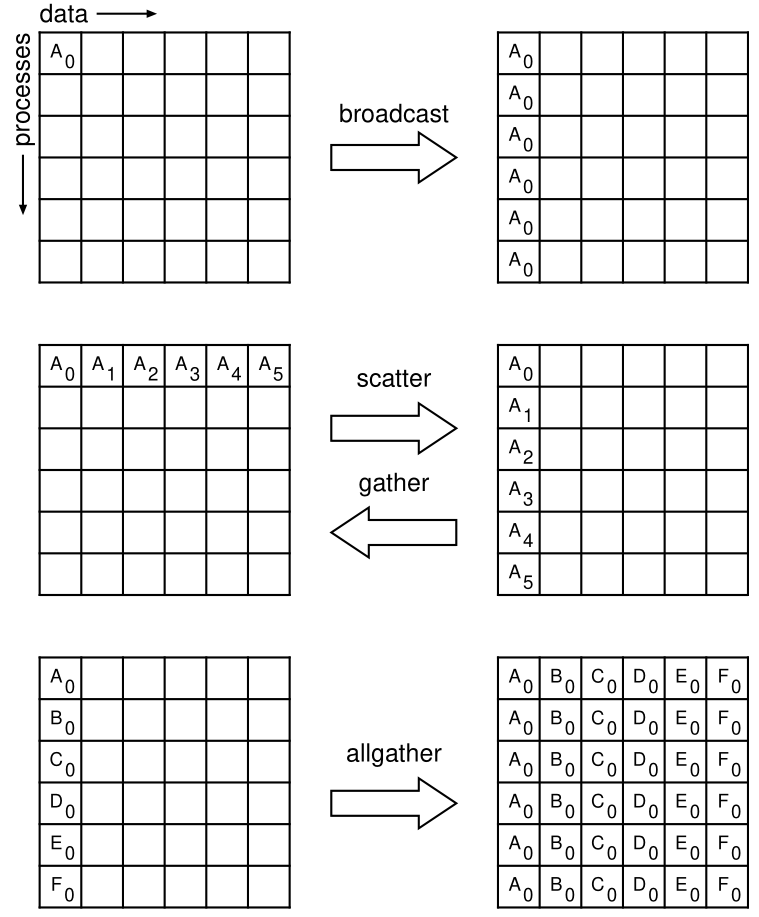
\includegraphics[width = 4.5in]{3_Chapters/2_Chapter_Background/Figs/mpispec_collective.png}
	\caption[Demonstration of collective communications]{
     Demonstration of collective communications taken from \cite{mpi40}.
     Columns specify each process' rank, and rows specify elements in the input vector.
     }
	\label{fig:mpispec_collectives}
\end{figure}

The reduction collectives, \texttt{MPI\_Reduce()} and \texttt{MPI\_Allreduce()}, are collectives of particular interest as they are heavily relied upon and tend to take up large parts of many application's run time.
Their defining characteristic is that they accept an operation which is applied to the data in flight.
\texttt{MPI\_Reduce()} is an all-to-one collective where each process specifies a buffer, and the result is placed at the root, while \texttt{MPI\_Allreduce()} is an all-to-all style collective where each process receives a copy of the final result. 
As an example, if each process had a double and the average across all doubles was necessary for the next step of the computation, each process could call \texttt{MPI\_Allreduce()} with a type \texttt{MPI\_DOUBLE} with the op \texttt{MPI\_SUM} to get the sum of each rank's double, and then divide the result by the communicator size to get the average.

Collective communications are considerably powerful as they can express a lot of data movement in a single operation, and for this reason, they are heavily used in production codes.
However, the inherent downside of collectives is the amount of synchronization they can introduce.
Collectives are not required to be blocking (except for \texttt{MPI\_Barrier}), but this is implementation dependant, and often the underlying algorithm can cause the calling process to stall.
Furthermore, since all processes in a communicator are required to participate, collectives often have the side effect of delaying early processes waiting for straggling processes to arrive.
Non-blocking collectives do exist, like the point-to-point interface, they return an \texttt{MPI\_Request} object that needs to be progressed with \texttt{MPI\_Test}/\texttt{MPI\_Wait}, but adoption is not that large and many codes still rely on blocking operations.

The popularity, yet simultaneous optimization challenges, have led to a large body of research on collective communication. 
There are also software packages that provide highly optimized collective communications outside of \gls{MPI}.
Notable examples include \gls{NCCL} \cite{NCCL}, which is designed to make optimal use of Nvidia's multi-\gls{GPU} servers, and \gls{UCC} \cite{UCC}, a modern library built on top of \gls{UCX}.
The internals of \gls{UCC} and \gls{NCCL} do not use \gls{MPI} primitives and have to reimplement a lot of wire-up and process orchestration handled within \gls{MPI}, however, their \gls{API}s are compatible with \gls{MPI}'s collective \gls{API}s, and \gls{MPI} implementations can leverage \gls{UCC} and \gls{NCCL} to perform collectives.
There are many strategies for optimizing collective algorithms, two of which we rely on for this thesis, including topology awareness in chapter \ref{ch:CH4-TopologyAwareness} and process arrival pattern awareness in chapter \ref{ch:CH5-PAPAwareness}.

\subsubsection{Algorithm Structure}\label{sec:CH2-MPI-AlgStructure}
Under the hood, collective algorithms are implemented as a series of point-to-point messages. 
There are different ways to structure the exchanges to implement a specified collective, and different structures have different performance tradeoffs depending on the collective's parameters.
One of the most impactful parameters in communication is the size of the message, and it is best exemplified through Hockney's model \cite{Hockney1994HockenyModel}.
Hockney's model states that the time to send a message of $n$ bytes can be estimated as $T_{msg}=\alpha+n\beta$, where $\alpha$ represents the startup overhead cost (seconds), and $\beta$ is inverse bandwidth (seconds per byte).
In practice, small messages are latency bound (dependent on $\alpha$), while large messages are bandwidth bound (dependent on $n\beta$).
This principle extends to collective algorithms, where designs fall into the same two categories, bandwidth bound and latency bound.
Thakur et al. \cite{Thakur2005OptMPICH} provide an analysis of the collective algorithms used in MPICH, leveraging Hockney's model to estimate collective performance.
Latency-bound algorithms try to minimize the number of messages sent as the fewer times we invoke $\alpha$, the faster the algorithm. 
In contrast, large message algorithms will break the data vector into components and issue multiple smaller messages, while this does increase the coefficient of $\alpha$, it minimizes the $n\beta$ coefficient, decreasing the total amount of data sent.
When dealing with reduction operations, we can add a $\gamma$ term representing the time to perform a reduction in seconds per flop, similar to the $\beta$, which scales with $n$.

\begin{figure}
    \centering
    \begin{tikzpicture}[auto]
    
        \def \bkxscale {1.25}
        \def \bkyscale {0.5}
        \begin{scope}[every node/.style={draw, rectangle}, minimum height=0.5cm, minimum width=1.25cm, font=\tiny]
            \foreach \y in {0,1,2,3} \foreach \x in {0,1,2,3} \node at (\x*\bkxscale,\y*\bkyscale) (a\x\y) {$ABCD_{0}$};
            \foreach \y in {10,11,12,13} \foreach \x in {0,1,2,3} \node at (\x*\bkxscale,\y*\bkyscale) (d\x\y) {};
            \foreach \y in {10,11,12,13} \foreach \x in {5,6,7,8} \node at (\x*\bkxscale,\y*\bkyscale) (e\x\y) {};
            \foreach \y\ly in {15/D,16/C,17/B,18/A} \foreach \x\lx in {0cm / 3,1cm / 2,2cm / 1,3cm / 0} \node at (\x*\bkxscale,\y*\bkyscale) (f\x\y) {$\ly_{\lx}$};
            \foreach \y in {15,16,17,18} \foreach \x in {5,6,7,8} \node at (\x*\bkxscale,\y*\bkyscale) (g\x\y) {};
        
            \draw[line width=1pt, double distance=3pt, arrows = {-Latex[length=0pt 3 0]}] (3.5*\bkxscale, 16.5*\bkyscale) -- (4.5*\bkxscale, 16.5*\bkyscale);
            \draw[line width=1pt, double distance=3pt, arrows = {-Latex[length=0pt 3 0]}] (3.5*\bkxscale, 11.5*\bkyscale) -- (4.5*\bkxscale, 11.5*\bkyscale);
            \draw[line width=1pt, double distance=3pt, arrows = {-Latex[length=0pt 3 0]}] (3.5*\bkxscale, 6.5*\bkyscale) -- (4.5*\bkxscale, 6.5*\bkyscale);
            \draw[line width=1pt, double distance=3pt, arrows = {-Latex[length=0pt 3 0]}] (4.5*\bkxscale, 14.5*\bkyscale) -- (3.5*\bkxscale, 13.5*\bkyscale);
            \draw[line width=1pt, double distance=3pt, arrows = {-Latex[length=0pt 3 0]}] (4.5*\bkxscale, 9.5*\bkyscale) -- (3.5*\bkxscale, 8.5*\bkyscale);
            \draw[line width=1pt, double distance=3pt, arrows = {-Latex[length=0pt 3 0]}] (4.5*\bkxscale, 4.5*\bkyscale) -- (3.5*\bkxscale, 3.5*\bkyscale);
            
            \node at (5*\bkxscale, 17*\bkyscale) (comebacktome) {$AB_0$};
            \node at (6*\bkxscale, 16*\bkyscale) (comebacktome) {$BC_1$};
            \node at (7*\bkxscale, 15*\bkyscale) (comebacktome) {$CD_2$};
            \node at (8*\bkxscale, 18*\bkyscale) (comebacktome) {$AD_3$};
            
            \node at (0*\bkxscale, 12*\bkyscale) (comebacktome) {$AB_0$};
            \node at (1*\bkxscale, 11*\bkyscale) (comebacktome) {$BC_1$};
            \node at (2*\bkxscale, 10*\bkyscale) (comebacktome) {$CD_2$};
            \node at (3*\bkxscale, 13*\bkyscale) (comebacktome) {$AD_3$};
            \node at (0*\bkxscale, 11*\bkyscale) (comebacktome) {$ABC_0$};
            \node at (1*\bkxscale, 10*\bkyscale) (comebacktome) {$BCD_1$};
            \node at (2*\bkxscale, 13*\bkyscale) (comebacktome) {$ACD_2$};
            \node at (3*\bkxscale, 12*\bkyscale) (comebacktome) {$ABD_3$};
            
            \node at (5*\bkxscale, 12*\bkyscale) (comebacktome) {$AB_0$};
            \node at (6*\bkxscale, 11*\bkyscale) (comebacktome) {$BC_1$};
            \node at (7*\bkxscale, 10*\bkyscale) (comebacktome) {$CD_2$};
            \node at (8*\bkxscale, 13*\bkyscale) (comebacktome) {$AD_3$};
            \node at (5*\bkxscale, 11*\bkyscale) (comebacktome) {$ABC_0$};
            \node at (6*\bkxscale, 10*\bkyscale) (comebacktome) {$BCD_1$};
            \node at (7*\bkxscale, 13*\bkyscale) (comebacktome) {$ACD_2$};
            \node at (8*\bkxscale, 12*\bkyscale) (comebacktome) {$ABD_3$};
            \node at (5*\bkxscale, 10*\bkyscale) (comebacktome) {$ABCD_0$};
            \node at (6*\bkxscale, 13*\bkyscale) (comebacktome) {$ABCD_1$};
            \node at (7*\bkxscale, 12*\bkyscale) (comebacktome) {$ABCD_2$};
            \node at (8*\bkxscale, 11*\bkyscale) (comebacktome) {$ABCD_3$};
            
            \node at (0*\bkxscale, 7*\bkyscale) (comebacktome) {$AB_0$};
            \node at (1*\bkxscale, 6*\bkyscale) (comebacktome) {$BC_1$};
            \node at (2*\bkxscale, 5*\bkyscale) (comebacktome) {$CD_2$};
            \node at (3*\bkxscale, 8*\bkyscale) (comebacktome) {$AD_3$};
            \node at (0*\bkxscale, 6*\bkyscale) (comebacktome) {$ABC_0$};
            \node at (1*\bkxscale, 5*\bkyscale) (comebacktome) {$BCD_1$};
            \node at (2*\bkxscale, 8*\bkyscale) (comebacktome) {$ACD_2$};
            \node at (3*\bkxscale, 7*\bkyscale) (comebacktome) {$ABD_3$};
            \node at (0*\bkxscale, 5*\bkyscale) (comebacktome) {$ABCD_0$};
            \node at (1*\bkxscale, 8*\bkyscale) (comebacktome) {$ABCD_1$};
            \node at (2*\bkxscale, 7*\bkyscale) (comebacktome) {$ABCD_2$};
            \node at (3*\bkxscale, 6*\bkyscale) (comebacktome) {$ABCD_3$};
            \node at (0*\bkxscale, 8*\bkyscale) (comebacktome) {$ABCD_0$};
            \node at (1*\bkxscale, 7*\bkyscale) (comebacktome) {$ABCD_1$};
            \node at (2*\bkxscale, 6*\bkyscale) (comebacktome) {$ABCD_2$};
            \node at (3*\bkxscale, 5*\bkyscale) (comebacktome) {$ABCD_3$};
            
            \node at (5*\bkxscale, 7*\bkyscale) (comebacktome) {$ABCD_0$};
            \node at (6*\bkxscale, 6*\bkyscale) (comebacktome) {$ABCD_1$};
            \node at (7*\bkxscale, 5*\bkyscale) (comebacktome) {$ABCD_2$};
            \node at (8*\bkxscale, 8*\bkyscale) (comebacktome) {$ABCD_3$};
            \node at (5*\bkxscale, 6*\bkyscale) (comebacktome) {$ABC_0$};
            \node at (6*\bkxscale, 5*\bkyscale) (comebacktome) {$BCD_1$};
            \node at (7*\bkxscale, 8*\bkyscale) (comebacktome) {$ACD_2$};
            \node at (8*\bkxscale, 7*\bkyscale) (comebacktome) {$ABD_3$};
            \node at (5*\bkxscale, 5*\bkyscale) (comebacktome) {$ABCD_0$};
            \node at (6*\bkxscale, 8*\bkyscale) (comebacktome) {$ABCD_1$};
            \node at (7*\bkxscale, 7*\bkyscale) (comebacktome) {$ABCD_2$};
            \node at (8*\bkxscale, 6*\bkyscale) (comebacktome) {$ABCD_3$};
            \node at (5*\bkxscale, 8*\bkyscale) (comebacktome) {$ABCD_0$};
            \node at (6*\bkxscale, 7*\bkyscale) (comebacktome) {$ABCD_1$};
            \node at (7*\bkxscale, 6*\bkyscale) (comebacktome) {$ABCD_2$};
            \node at (8*\bkxscale, 5*\bkyscale) (comebacktome) {$ABCD_3$};
            
        \end{scope}
        
    \end{tikzpicture}
    \caption[Outline of ring allreduce algorithm]{
        Ring allreduce algorithm. Each grid represents a step in the algorithm, where rows are ranks and columns are segments of the data vector.
    }
    \label{fig:ring-allreduce-grid} 
\end{figure}
Figure \ref{fig:ring-allreduce-grid} outlines a four-rank ring allreduce.
The ring algorithm is often used for large message allreduce because its bandwidth-based performance scales linearly.
To perform the algorithm, each rank receives data from a neighbouring rank and forwards it to the next, and in essence, data is propagated around the communicator in a giant ring.
Formally, each rank $r$ sends a message to rank $(r+1) \% comm\_size$ and receives a message from rank $(r-1+comm\_size) \% comm\_size$, where the modulo term enforces a wrap-around so rank 0 and rank $p-1$ exchange data.
For a ring of $p$ processes, the first $p-1$ steps consist of a data exchange and reduction operation, where each chunk of data consists of $n/p$ bytes of data. 
At the midway point (the fourth grid in Figure \ref{fig:ring-allreduce-grid}), each rank will hold $1/n$ of the fully reduced vector, this data distribution can be considered a reduce-scatter.
The algorithm finishes with another $p-1$ exchanges of size $n/p$, this time without the reduce, which acts as an allgather distributing the final result.
In total, $2(p-1)$ messages of size $n/p$ are sent, with half of them requiring a reduction, and this can give us a total collective time of $T_{ring} = 2(p-1)\alpha + 2((p-1)/p)n\beta + ((p-1)/p)n\gamma$.

The ring algorithm can be generalized to a reduce-scatter followed by an allgather and maintains the $2(p-1)/p)n\beta$ term.
This leads to another popular implementation of allreduce, the \gls{RSA} algorithm, also known as Rabenseifner's algorithm.
This method breaks the vector into chunks and uses a recursive doubling method to complete the operation in a logarithmic number of steps.
The most common implementation, outlined in Figure \ref{fig:rsa-allreduce-grid}, uses distance doubling/vector halving to implement reduce-scatter and distance halving/vector doubling to implement allgather \cite{Rabenseifner2004OptOfCollRedOps}.
The reduce-scatter starts by sending half the vector to an immediate neighbour, then doubles the distance and halves the data for the next $log(p)$ steps of the reduce-scatter.
The allgather takes the reverse approach, it receives $1/p$ Bytes of data from a rank $p/2$ away, then doubles the data every step while halving the distance to its partner.
This maintains the same bandwidth term as the ring algorithm but lowers the number of messages to $2\log(p)$, however, extra steps may be required if $p$ is not a power of 2.
\begin{figure}
    \centering
    \begin{tikzpicture}[
        hasty/.style={draw,single arrow, minimum height=1cm, minimum width=0.2cm},
        dasty/.style={draw,single arrow, minimum height=1cm, minimum width=0.2cm,rotate=-150},
        bsty/.style={draw, rectangle, minimum height=0.5cm, minimum width=1.25cm, font=\tiny},
        fsty/.style={font=\tiny},
    ]
    
        \def \bkxscale {1.25}
        \def \bkyscale {0.5}
            \foreach \y\ly in {15/D,16/C,17/B,18/A} 
                \foreach \x\lx in {0cm / 0,1cm / 1,2cm / 2,3cm / 3} 
                    \node[bsty] at (\x*\bkxscale,\y*\bkyscale) (f\x\y) {$\ly_{\lx}$};
            \foreach \y in {10,11,12,13} 
                \foreach \x in {0,1,2,3} 
                    \node[bsty] at (\x*\bkxscale,\y*\bkyscale) (d\x\y) {};
            \foreach \y in {10,11,12,13} 
                \foreach \x in {5,6,7,8} 
                    \node[bsty] at (\x*\bkxscale,\y*\bkyscale) (e\x\y) {};
            \foreach \y in {15,16,17,18} 
                \foreach \x in {5,6,7,8}
                    \node[bsty] at (\x*\bkxscale,\y*\bkyscale) (g\x\y) {};
            \foreach \y in {5,6,7,8}
                \foreach \x in {0,1,2,3}
                    \node[bsty] at (\x*\bkxscale,\y*\bkyscale) (a\x\y) {$ABCD_{0}$};

            \node[] at (-0.2*\bkxscale, 20*\bkyscale) (ld) {Data}; 
            \draw[->] (ld) -- (1.2*\bkxscale, 20*\bkyscale);
            \foreach \x in {0,1,2,3}
                \node at (\x*\bkxscale, 19*\bkyscale) () {\x};
            \foreach \x/\l in {5/0,6/1,7/2,8/3}
                \node at (\x*\bkxscale, 19*\bkyscale) () {\l};
                
            \node[rotate=90] at (-1.2*\bkxscale, 17.7*\bkyscale) (lr) {Rank}; 
            \draw[->] (lr) -- (-1.2*\bkxscale, 15.7*\bkyscale);
            \foreach \y/\l in {15/D,16/C,17/B,18/A} 
                \node at (-0.8*\bkxscale, \y*\bkyscale) () {$r_\l$};
            \foreach \y/\l in {10/D,11/C,12/B,13/A} 
                \node at (-0.8*\bkxscale, \y*\bkyscale) () {$r_\l$};
            \foreach \y/\l in {5/D,6/C,7/B,8/A} 
                \node at (-0.8*\bkxscale, \y*\bkyscale) () {$r_\l$};
            % \foreach \y/\l in {0/D,1/C,2/B,3/A} 
            %     \node at (-0.8*\bkxscale, \y*\bkyscale) () {$r_\l$};
            

            \node[hasty] at (4*\bkxscale, 16.5*\bkyscale) (){};
            \node[dasty] at (4*\bkxscale, 14*\bkyscale) (){};
            \node[hasty] at (4*\bkxscale, 11.5*\bkyscale) (){};
            \node[dasty] at (4*\bkxscale, 9*\bkyscale) (){};
            % \node[hasty] at (4*\bkxscale, 6.5*\bkyscale) (){};
            % \node[dasty] at (4*\bkxscale, 4*\bkyscale) (){};
            
            \node[fsty] at (5*\bkxscale, 18*\bkyscale) () {$AB0$};
            \node[fsty] at (6*\bkxscale, 18*\bkyscale) () {$AB_1$};
            \node[fsty] at (5*\bkxscale, 16*\bkyscale) () {$CD_0$};
            \node[fsty] at (6*\bkxscale, 16*\bkyscale) () {$CD_1$};
            \node[fsty] at (7*\bkxscale, 17*\bkyscale) () {$AB_2$};
            \node[fsty] at (8*\bkxscale, 17*\bkyscale) () {$AB_3$};
            \node[fsty] at (7*\bkxscale, 15*\bkyscale) () {$CD_2$};
            \node[fsty] at (8*\bkxscale, 15*\bkyscale) () {$CD_3$};
            
            \node[fsty] at (0*\bkxscale, 13*\bkyscale) () {$ABCD_0$};
            \node[fsty] at (1*\bkxscale, 13*\bkyscale) () {$AB_1$};
            \node[fsty] at (0*\bkxscale, 11*\bkyscale) () {$CD_0$};
            \node[fsty] at (1*\bkxscale, 11*\bkyscale) () {$ABCD_1$};
            \node[fsty] at (2*\bkxscale, 12*\bkyscale) () {$ABCD_2$};
            \node[fsty] at (3*\bkxscale, 12*\bkyscale) () {$AB_3$};
            \node[fsty] at (2*\bkxscale, 10*\bkyscale) () {$CD_2$};
            \node[fsty] at (3*\bkxscale, 10*\bkyscale) () {$ABCD_3$};
            
            \node[fsty] at (5*\bkxscale, 13*\bkyscale) () {$ABCD_0$};
            \node[fsty] at (6*\bkxscale, 13*\bkyscale) () {$ABCD_1$};
            \node[fsty] at (5*\bkxscale, 11*\bkyscale) () {$ABCD_0$};
            \node[fsty] at (6*\bkxscale, 11*\bkyscale) () {$ABCD_1$};
            \node[fsty] at (7*\bkxscale, 12*\bkyscale) () {$ABCD_2$};
            \node[fsty] at (8*\bkxscale, 12*\bkyscale) () {$ABCD_3$};
            \node[fsty] at (7*\bkxscale, 10*\bkyscale) () {$ABCD_2$};
            \node[fsty] at (8*\bkxscale, 10*\bkyscale) () {$ABCD_3$};
            
        
    \end{tikzpicture}
    \caption[RSA Allreduce Algorithm]{
        An implementation of the RSA allreduce algorithm using distance doubling/vector halving.
        Each grid represents a step in the algorithm, where rows are ranks and columns are segments of the data vector.
    }
    \label{fig:rsa-allreduce-grid} 
\end{figure}

One-to-all type collective algorithms can often be modelled as trees where vertices are ranks, edges between vertices are messages, and the root of the tree is the root of the collective.
The structure of the tree will have an impact on collective time, for example, a binary tree would theoretically perform better than a linear tree (also known as a chain) due to the logarithmic nature of its height.
Collective algorithms can also leverage message pipelining techniques, where a message is broken into segments and propagated through a tree letting different segments overlap.
By default, a chain broadcast would take $T_{chain}=p\alpha+pn\beta$, but with a segment size of $k$ it could be performed in $T_{chain\_pipe}=(n/k+p-1)\alpha+(n+(p-2)k)\beta$.
Pipelining leverages concurrency by propagating data through multiple stages of the tree parallel and shows the most benefit for large message collectives.

While many of these algorithms are foundational to collective research, they tend to make several naive assumptions about the underlying hardware.
Topology-awareness breaks the assumption that all messages cost the same.
As outlined in \ref{sec:CH2-interconnects}, different interconnects have different performance characteristics, and it has been shown that adapting the collective structure to the underlying hardware can unlock a lot of performance. 
One other assumption is that all processes arrive at the same time, and process-arrival-pattern-aware collectives break this assumption, they look at how data dependencies within a communication structure can be decoupled to unlock performance.

\subsubsection{Topology Awareness}
Topology awareness, as the name implies, revolves around passing hardware information to the runtime to use resources intelligently.
To perform this task, the \gls{MPI} runtime needs two pieces of information: system hardware information and application communication information.
The hardware info encompasses how processing elements are interconnected and includes the host memory characteristics (\gls{NUMA} and cache hierarchies), \gls{PCIe} information on how devices and \gls{CPU}s are connected, and network characteristics like topology or routing strategy.
This info is relatively easy to collect.
There are several libraries for exposing this info to applications, and many \gls{MPI} implementations already collect this information at runtime.

Acting on topology information is a whole different kind of challenge, as these problems involve modelling an application's communication and accelerating it with the hardware info, and many methods have been attempted over the years.
There are ahead-of-time mapping methods, which involve measuring all communication during a profiling run of an application, using the logs to model a communication pattern, and using the communication pattern to calculate an optimal process to core binding before all future runs of the application \cite{Hoefler2011GenericTopoMappingStrats,Mirsadeghi2016PTRAM}. 
There are runtime-based methods, like virtual topologies, where applications can pass hints to the \gls{MPI} runtime indicating how communication will be structured across a communicator \cite{Gropp2019CartTopoMapping}.
Virtual topologies can include multidimensional cartesian grids or user-specified graphs, and the \gls{MPI} implementation can leverage topology information to more optimally assign ranks in the new communicator.
Collectives are also a target for topology awareness, as the collective specifies the expected communication, and the implementation is given free rein to optimize the algorithm however it sees fit \cite{Mirsadeghi2016TopoAwareCollRR, Luo2018ADAPT}.

One noteworthy class of topology-aware collective algorithms are hierarchical algorithms \cite{Chu2020NVGroup}.
System topologies can often be broken into hierarchies based on performance, where common groupings often include cache layers, \gls{NUMA} domains, and levels of a fat-tree network.
Using flat algorithms as building blocks, hierarchical collectives compose cluster-wide collectives through small-scale collectives performed with subsets of the larger communicator on different layers of the hierarchy.
Each grouping on a hierarchical layer will select a leader responsible for communicating across higher hierarchies.
The most basic hierarchy relies on an intranode communicator, where all ranks are on the same node, and an internode communicator, where every rank is on a different node.
Figure \ref{fig:sample_heir_allreduce} demonstrates a typical two-layer hierarchical allreduce which is performed in 4 steps: 1) intranode reduce to the leader, 2) internode reduce to some predetermined rank, 3) internode broadcast and 4) intranode broadcast.
These algorithms rely on topology information to build hierarchies and are structured to maximize the amount of traffic on performant interconnects while minimizing the amount of traffic on slower links.

\begin{figure}
    \centering
    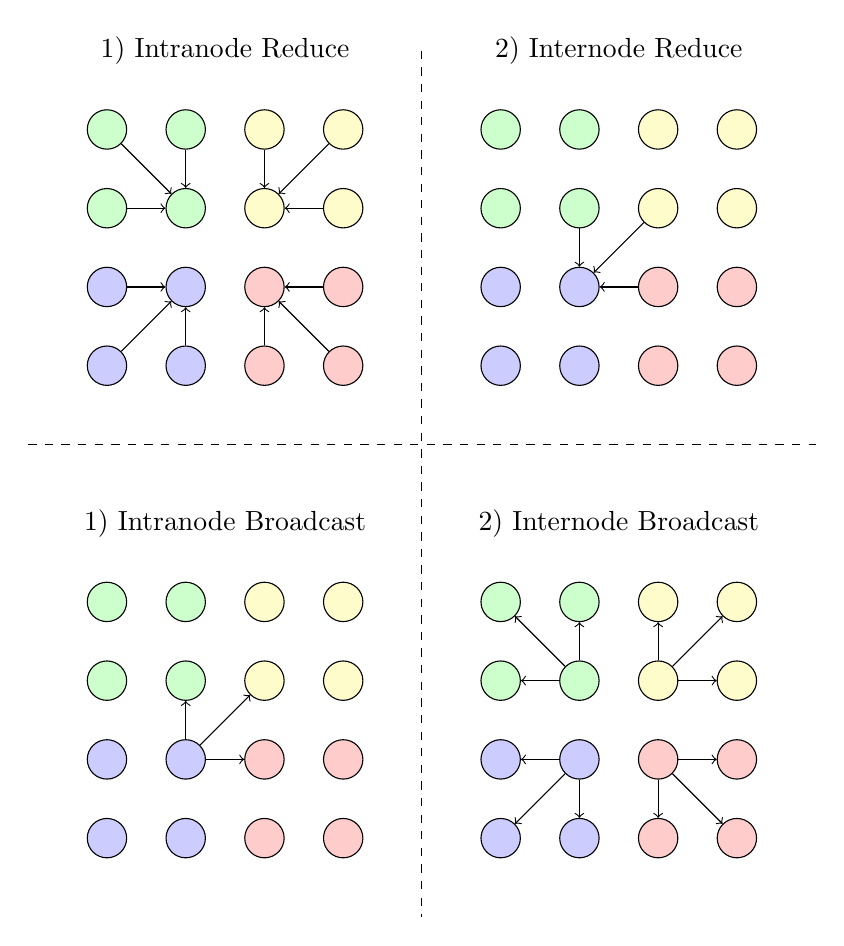
\begin{tikzpicture}[
        nsty/.style={
            draw,circle,
            minimum height=0.5cm,
        },
        csty0/.style={fill=blue!20},
        csty1/.style={fill=green!20},
        csty2/.style={fill=red!20},
        csty3/.style={fill=yellow!20},
    ]
    
    \foreach \n/\ox/\oy in {0/0/6,1/0/8,2/2/6,3/2/8}{
        \node[nsty,csty\n] at (\ox, \oy) (a0\n) {};
        \node[nsty,csty\n] at (1+\ox,\oy) (a1\n) {};
        \node[nsty,csty\n] at (\ox,1+\oy) (a2\n) {};
        \node[nsty,csty\n] at (1+\ox,1+\oy) (a3\n) {};
    }
    \draw[->] (a00) -- (a30);
    \draw[->] (a10) -- (a30);
    \draw[->] (a20) -- (a30);
    \draw[->] (a01) -- (a11);
    \draw[->] (a21) -- (a11);
    \draw[->] (a31) -- (a11);
    \draw[->] (a02) -- (a22);
    \draw[->] (a12) -- (a22);
    \draw[->] (a32) -- (a22);
    \draw[->] (a13) -- (a03);
    \draw[->] (a23) -- (a03);
    \draw[->] (a33) -- (a03);
    
    \foreach \n/\ox/\oy in {0/5/6,1/5/8,2/7/6,3/7/8}{
        \node[nsty,csty\n] at (\ox, \oy) (b0\n) {};
        \node[nsty,csty\n] at (1+\ox,\oy) (b1\n) {};
        \node[nsty,csty\n] at (\ox,1+\oy) (b2\n) {};
        \node[nsty,csty\n] at (1+\ox,1+\oy) (b3\n) {};
    }
    \draw[->] (b11) -- (b30);
    \draw[->] (b22) -- (b30);
    \draw[->] (b03) -- (b30);

    \foreach \n/\ox/\oy in {0/0/0,1/0/2,2/2/0,3/2/2}{
        \node[nsty,csty\n] at (\ox, \oy) (c0\n) {};
        \node[nsty,csty\n] at (1+\ox,\oy) (c1\n) {};
        \node[nsty,csty\n] at (\ox,1+\oy) (c2\n) {};
        \node[nsty,csty\n] at (1+\ox,1+\oy) (c3\n) {};
    }
    \draw[<-] (c11) -- (c30);
    \draw[<-] (c22) -- (c30);
    \draw[<-] (c03) -- (c30);

    
    \foreach \n/\ox/\oy in {0/5/0,1/5/2,2/7/0,3/7/2}{
        \node[nsty,csty\n] at (\ox, \oy) (d0\n) {};
        \node[nsty,csty\n] at (1+\ox,\oy) (d1\n) {};
        \node[nsty,csty\n] at (\ox,1+\oy) (d2\n) {};
        \node[nsty,csty\n] at (1+\ox,1+\oy) (d3\n) {};
    }
    \draw[<-] (d00) -- (d30);
    \draw[<-] (d10) -- (d30);
    \draw[<-] (d20) -- (d30);
    \draw[<-] (d01) -- (d11);
    \draw[<-] (d21) -- (d11);
    \draw[<-] (d31) -- (d11);
    \draw[<-] (d02) -- (d22);
    \draw[<-] (d12) -- (d22);
    \draw[<-] (d32) -- (d22);
    \draw[<-] (d13) -- (d03);
    \draw[<-] (d23) -- (d03);
    \draw[<-] (d33) -- (d03);

    \draw[dashed] (4,10) -- (4,-1);
    \draw[dashed] (-1,5) -- (9,5);
    \node[align=center] at (1.5, 10) {1) Intranode Reduce}; 
    \node[align=center] at (6.5, 10) {2) Internode Reduce}; 
    \node[align=center] at (1.5, 4) {1) Intranode Broadcast}; 
    \node[align=center] at (6.5, 4) {2) Internode Broadcast}; 
    
    \end{tikzpicture}
    \caption[Sixteen-Process Four-Node Hierarchical Allreduce]{
        A two-level hierarchical allreduce with 16 processes on 4 nodes, each colour representing a different node.
        The algorithm takes 4 steps, 1) intranode reduce, 2) internode reduce, 3) intranode broadcast, and 4) intranode broadcast.
    }
    \label{fig:sample_heir_allreduce}
\end{figure}

\subsubsection{Process Arrival Pattern Awareness}
 Another unique way of optimizing collective communications is to use \gls{PAP} awareness.
 \gls{PAP} awareness leverages process skew to mitigate performance loss or improve application performance. 
Most collective algorithms assume that all ranks enter the collective simultaneously, but in reality, performance is not deterministic.
Many stochastic factors, like OS process scheduling, network noise, and opportunistic \gls{CPU} frequency boosting can affect compute performance, and since they are random, they affect different ranks to different degrees.
All these factors can add a skew causing processes to arrive at different times \cite{Faraj2008StudyProcArrivalMPIColl}.

\begin{figure}
    \centering
    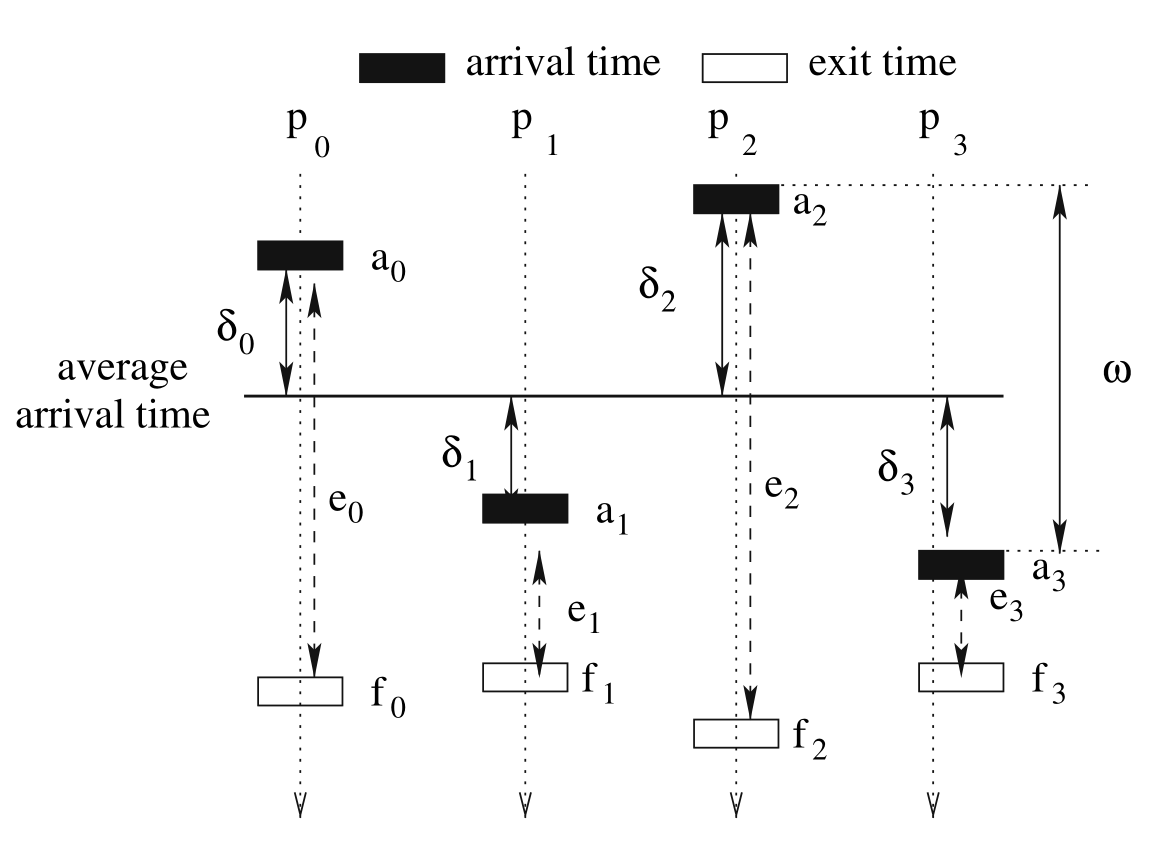
\includegraphics[width=4.5in]{3_Chapters/2_Chapter_Background/Figs/pap_theory.png}
    \caption[Outline of process arrival patterns theory]{
        An outline of process arrival pattern theory for four processes, taken from \cite{Faraj2008StudyProcArrivalMPIColl}.
    }
    \label{fig:pap-theory}
\end{figure}

Faraj et al. \cite{Faraj2008StudyProcArrivalMPIColl} provide a set of formal definitions for modelling process arrivals, a visual interpretation is given in Figure \ref{fig:pap-theory}.
For processes $(p_0, p_1,...,p_n)$ participating in a collective operation, each process has an arrival time denoted by $a_i$ and an exit time at $f_n$.
Therefore, each collective call has an arrival patterns $(a_0, a_1, ..., a_n)$ and an exit pattern $(f_0, f_1, ..., f_n)$.
Each rank spends $e_i = f_i - a_i$ time in the collective, where total collective time can be expressed as $e_0 + e_1 + ... + e_n$ and the average collective time is $\bar{e} = (e_0 + e_1 + ... + e_n)/n$.
Both the average and total collective are useful in evaluating the overall collective performance.
To quantify the difference between process arrivals, let $\delta_i$ be the absolute time difference between a process's arrival and the average arrival time, i.e., $\delta_i = |\bar{a} - a_i|$. 
We can then define the average arrival imbalance as $\bar{\delta}=(\delta_0 + \delta_i + ... + \delta_n)/n$, and the maximum imbalance time as $\omega = max_i(a_i)-min_i(a_i)$.
When using average/max imbalance in practice, it is often easier to normalize it by the message transmission time.
If the time to send a message of $n$ bytes is $T$, then the \gls{MIF} for that message is $\omega/T$, and the \textit{average imbalance factor} is $\bar{\delta}/T$.

To apply this theory to actual collectives, several problems must be solved.
One of the predominant issues with \gls{PAP}-Awareness is determining the \gls{PAP}.
Each process needs arrival information to determine its position relative to its peers so that it can take appropriate action within the collective algorithm. 
One strategy for inter-node \gls{PAP} awareness can include exchanging control messages using \gls{MPI} point-to-point routines leveraging \texttt{MPI\_ANY\_SOURCE} \cite{Patarasuk2008EffBcastDifProcArr}.
These strategies are not ideal, as these mechanisms require the active participation of some leader processes.
This is often delegated to the root in one-to-many or many-to-one collectives, but does not map as easily to many-to-many collectives.
Further, this adds overhead and worsens workload imbalance as one process spends considerably more cycles orchestrating process arrival information.
There is also the issue of processes stalling before the root has arrived, as no work can be done before \gls{PAP} information is exchanged.
Some proposed work fixes this by delegating \gls{PAP} management to a background thread \cite{Proficz2018ImprvAllReduceForImbPAP, Proficz2020PAPAwareScatterGather, Proficz2021AllGatherResilientToImbPAP, Faraj2008StudyProcArrivalMPIColl}, but this solution can add more imbalance due to thread scheduling, as well as a burden on application developers to manage resources of background threads.
Other internode solutions rely on non-portable interfaces like \gls{RDMA} verbs on InfiniBand \cite{Qian2009ProcArrivalSHMA2AIB}.
Since one-sided operations do not require remote host involvement, they allow early processes to exchange data with late processes, but locking the solution into specific hardware is not ideal.

